% ---------------------------------------------------------
% Project: PhD KAPPA
% File: results.1.tex
% Author: Andrea Discacciati
%
% Purpose: Paper I (results)
% ---------------------------------------------------------

\section{Paper I}

In this paper we examined the association of BMI during early adulthood (30 years of age) and middle-late adulthood (45--79 years of age) with  the incidence of prostate cancer subtypes and with prostate cancer mortality in the population-based COSM.

\subsection{Main results}

Baseline age-standardized characteristics of the study participants according to categories of BMI during middle-late adulthood are presented in \citetalias[table 1]{discacciati_body_2011}. Overweight and obese men at baseline were more likely to have a personal history of diabetes and to be former smokers as compared with underweight and normal-weight men. On the other hand, they were less likely to be physically active or well-educated.

Multivariable-adjusted IRRs and MRRs according to levels of BMI at baseline age and BMI at age 30 years are presented in \citetalias[table~2, table~3, and figure~1.]{discacciati_body_2011}

For localized prostate cancer, BMI at baseline age was modeled using the best-fitting FP2 transformation, which was characterized by fractional powers $(-2, -2)$. This increased the overall fit of the model as compared with modeling BMI in a linear fashion ($\mathrm{AIC}_{\textrm{FP2}(-2,-2)} = 36614$ versus $\mathrm{AIC}_{\textrm{linear}} = 36616$), and conferred to the relationship between BMI at baseline age and IR of localized prostate cancer an inverse--U shape. In particular, the IR of localized prostate cancer at 35 \kgmsq{} was 29\% lower than that at 22 \kgmsq{} [IRR: 0.71 (95\% CI: 0.53--0.94)], while the IR at 18 \kgmsq{} was 12\% lower [IRR: 0.78 (95\% CI: 0.54--1.13)]. BMI at age 30 years was associated with a 2\% decreased IR for every 5-unit increment [IRR: 0.98 (95\% CI: 0.87--1.12)].

For advanced prostate cancer, BMI at baseline age was associated with a 4\% increased IR [IRR: 1.04 (95\% CI: 0.88--1.22)], whereas BMI at age 30 years was associated with a 10\% decreased IR [IRR: 0.90 (95\% CI: 0.73--1.11)], both for every 5-unit increment.

For fatal prostate cancer, BMI at baseline age was associated with a 12\% increased MR [MRR: 1.12 (95\% CI: 0.87--1.43)], while BMI at age 30 years was associated with a 27\% decreased MR [MRR: 0.73 (95\% CI: 0.53--1.02)], both for every 5-unit increment.

\subsection{Updated analyses with extended follow-up}
\label{section:updated_paper1}

For localized prostate cancer, BMI at baseline age showed an inverse--U association, regardless of whether it was modeled using FP2$(-2, -2)$ (green line),  FP2$(-1, 0.5)$ (purple line),\footnote{The best-fitting FP2 in the updated data according to AIC.} or RCS (blue line) (figure \ref{fig:paper1_1997}). From the categorical analysis, the multivariable-adjusted IR for the obese men at baseline  (BMI $\ge30$ \kgmsq{}) was 21\% lower that that for men in the referent category (21.0--22.9 \kgmsq{}) [IRR: 0.79 (95\% CI: 0.64-0.98)] (table \ref{table:paper1_1997}). %BMI at age 30 was associated with a 0.3\% increased IR for every 5-unit increment [IRR: 1.003 (95\% CI: 0.90--1.12)] (table \ref{table:paper1_30} and figure \ref{fig:paper1_30}).

For advanced prostate cancer, BMI at baseline age was associated with a 11\% increased IR for every 5-unit increment [IRR: 1.11 (95\% CI: 0.96--1.27)] (table \ref{table:paper1_1997}). No evidence of non-linearity was observed from the RCS model ($p_{\textrm{non-linearity}}=0.30$) (figure \ref{fig:paper1_1997}). %while BMI at age 30 years was associated with a 9\% decreased IR [IRR: 0.91 (95\% CI: 0.76--1.10)], both for every 5-unit increment (table \ref{table:paper1_30} and figure \ref{fig:paper1_30}).

For fatal prostate cancer, BMI at baseline age was associated with a 12\% increased MR for every 5-unit increment [MRR: 1.12 (95\% CI: 0.95--1.32)] (table \ref{table:paper1_1997}). Again, no evidence of non-linearity was observed ($p_{\textrm{non-linearity}}=0.49$) (figure \ref{fig:paper1_1997}). %, whereas BMI at age 30 years was associated with a 16\% decreased MR [MRR: 0.84 (95\% CI: 0.68--1.05)], both for every 5-unit increment (table \ref{table:paper1_30} and figure \ref{fig:paper1_30}).

\begin{figure}[t]
\centering
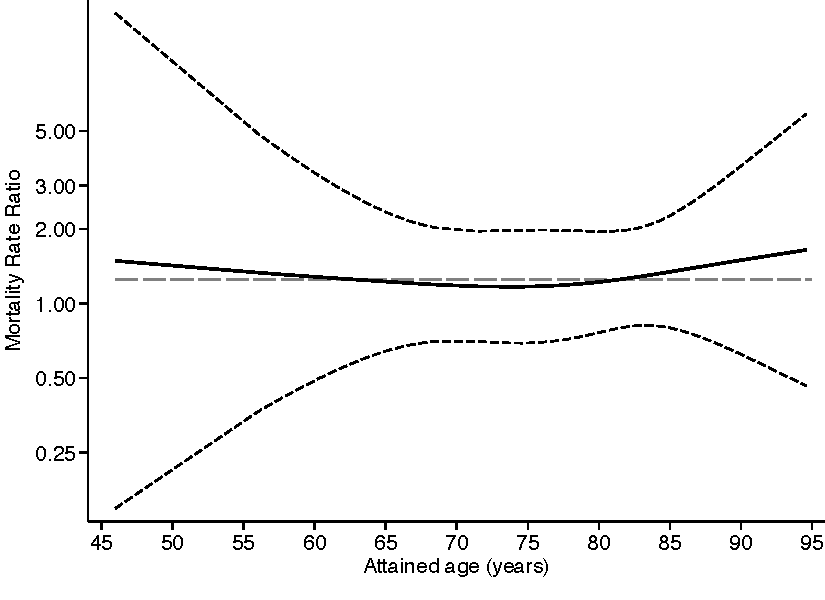
\includegraphics[width=.8\linewidth]{figures/tvcoef.pdf}
\caption[Time-varying Mortality Rate Ratio for BMI at baseline age $\ge$ 30 \kgmsq{}]{Time-varying MRR from prostate cancer for BMI at baseline age $\ge$ 30 \kgmsq{} versus 21.0--22.9 \kgmsq{} (solid black line). The dashed black lines are  95\% confidence interval. The long-dashed grey line is the time-fixed MRR, equal to 1.25 (table \ref{table:paper1_1997}). The vertical axis is on the natural log scale.}
\label{fig:tvcoef}
\end{figure}

No evidence against the PH assumption was observed for any of the exposure-outcome associations. For example, figure \ref{fig:tvcoef} shows the time-varying MRR of fatal prostate cancer for   BMI at baseline age $\ge$ 30 \kgmsq{} versus 21.0--22.9 \kgmsq{}, where the time-dependent coefficient for BMI was modeled using RCS with 3 knots placed at the the 10th, 50th, and 90th percentiles of the distribution of the uncensored event times \citep{discacciati_stphcoxrcs_2015}.\footnote{Corresponding to 65.5, 79.8, and 87.2 years of attained age.} The $p$-value relative to the test against the null hypothesis $H_0:\gamma_1=\gamma_2=0$ was equal to 0.91 [see equation (\ref{eq:timevcoef})].  

Lastly, no evidence of heterogeneity by county of residence at baseline  was observed, as shown in table \ref{table:paper1_heterogeneity}.

Updated results for BMI at 30 years of age are reported in table \ref{table:paper1_30} and in figure \ref{fig:paper1_30}. Overall, the results based on the updated data were consistent with those reported in \citetalias{discacciati_body_2011}, and generally more precise.

\begin{table}[h]
\centering
\begin{threeparttable}
\caption[Heterogeneity by county of residence in the associations between BMI at baseline age and localized, advanced, and fatal prostate cancer]{Heterogeneity by county of residence at baseline (Västmanland/Örebro) in the association between BMI at baseline age and localized, advanced, and fatal prostate cancer}
\label{table:paper1_heterogeneity}
\begin{tabular}{lccc}
\hline
\multicolumn{4}{c}{{\bf BMI at baseline age}}                                                    \\ \hline
{\bf Outcome}             & {\bf Västmanland} & {\bf Örebro}      & $p_{\textrm{heterogeneity}}$ \\ \hline
Localized prostate cancer\tnote{a} & 0.68 (0.44--0.91)  & 0.74 (0.49--1.00) & 0.35                         \\
Advanced prostate cancer\tnote{b}  & 1.13 (0.95--1.35) & 1.08 (0.90--1.30) & 0.71                         \\
Fatal prostate cancer\tnote{c}     & 1.20 (0.96--1.51) & 1.05 (0.85--1.30) & 0.36                         \\ \hline
\end{tabular}
\begin{tablenotes}
\item [a] \footnotesize Multivariable-adjusted IRR comparing a BMI of 35 \kgmsq{} with a BMI of 22 \kgmsq{} from the FP2$(-2,-2)$ model.
\item [b] \footnotesize Multivariable-adjusted IRR for every 5-unit increment.
\item [c] \footnotesize Multivariable-adjusted MRR for every 5-unit increment.
\end{tablenotes}
\end{threeparttable}
\end{table}

\begin{figure}[p]
\centering
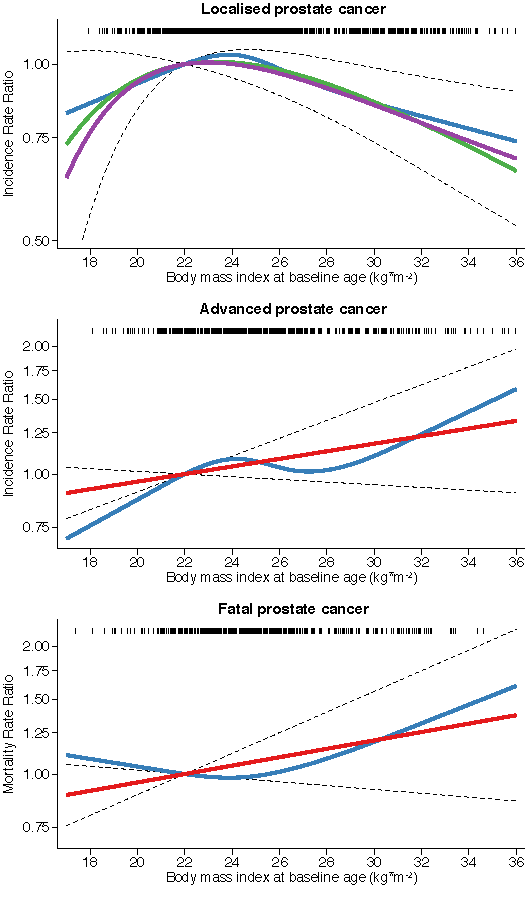
\includegraphics[width=.85\linewidth]{figures/paper1_1997.pdf}
\caption[Associations of BMI at baseline age with localized, advanced, and fatal prostate cancer]{Multivariable-adjusted associations of BMI at baseline age (\kgmsq) with IR of localized and advanced prostate cancer, and with MR of fatal prostate cancer in the updated analysis of \citetalias{discacciati_body_2011}. BMI was modeled using FP2$(-2,-2)$ (green line), FP2$(-1,0.5)$ (purple line), RCS with 4 knots (blue line), and in a linear fashion (red line).  The referent value was set at 22 \kgmsq. Vertical lines above the curves represent cases of prostate cancer. The vertical axes are on the natural log scale.}
\label{fig:paper1_1997}
\end{figure}



